\section{Method}

\subsection{Global Warming}

A function called global\_warming.C was created in C++, and was later executed in root. The function included the scripts "treader.h" and "tpoint.h" which were used to read the data provided. Three arguments were required, a path to the data file, and starting year and an end year for the analyze. The function then analyzed the data and calculated an average temperature for each year. A total average for all the used data was also calculated. Two histograms were then created, one colored red that contained all years above the total average and one colored blue that contained all years below the average. Two moving averages were also calculated using 

\section{Results}

\subsection{Global Warming}

The function was used with all the data contributed from Uppsala, i.e. temperature measurements from 1722 to 2013. A histogram including all the data was hence created,  see figure \ref{global_warming_figure}. The average temperature of each year was displayed as a bin stretching from the total average temperature of all the data. Red bins were used for bins with temperatures above the total average and blue bins were used otherwise. On top of this two graphs were created to show two types of moving averages. The first graph displayed an average calculated every 5 years by including the next and the previous 5 years (if any). The second graph was instead calculated every 10 years and included the next and the previous 20 years (if any). This graph was drawn with a thicker line in order to separate the two.

\begin{figure}[H]
\centering
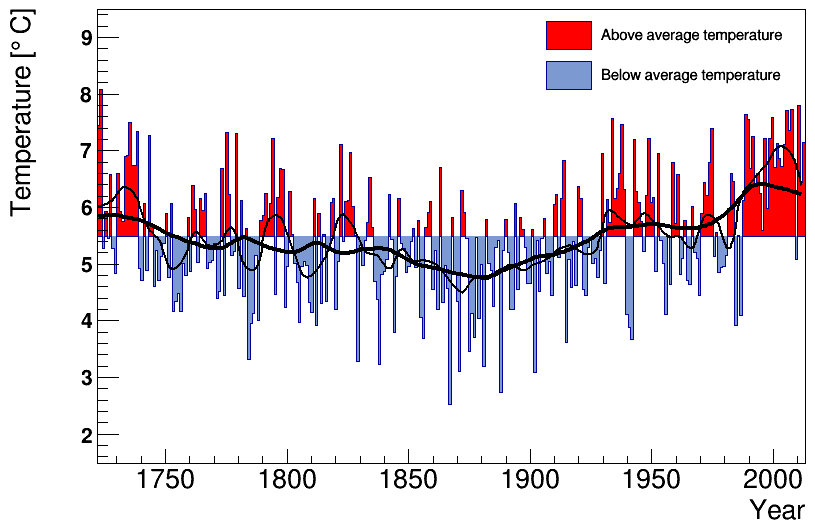
\includegraphics[width=0.9\textwidth]{global_warming.png}
\caption{\label{global_warming_figure} The average temperature of each year in Uppsala. A total average is calculated as $\approx 5.5 \hspace{1mm} ^\circ C$ and each average temperature is displayed as either a red bin, if the temperature is above the total average, or a blue bin, if the temperature is below the total average. Two black graphs displays moving averages. The thinner line describes the average in the vicinity of 5 years and the thicker line the vicinity of 20 years. Note that the average temperature of the last 20 years is disturbingly high. }
\end{figure}

\section{Discussion}

\subsection{Global Warming}

It is quite evident from the histogram (see figure \ref{global_warming_figure}) that the average temperature (at least in Uppsala) can vary a lot from one year to the next. Over decades however we can see a shift between warmer and colder periods, and even clearer if we observe the moving averages. The nineteenth century seem to have been quite a cold period in Sweden, with the average temperature dropping to almost one degree below the total average. The early eighteenth century may seem to indicate a higher average, but this is mostly due to that the years 1722 to 1735 were all quite warm, and the moving average has no data prior to 1722 to use. It is hence unclear whether the average temperature of the eighteenth century was much higher than that of the following century, and the moving averages might be a bit misleading in this regard.

From the histogram it is more evident that the average temperature since the start of the twentieths century has increased. The average temperature between 1970 and 2010 is more than a degree higher than that of the period between 1870 and 1910. This does not prove any form of man-made global warming, but it is a strong indication that the surface-temperature of the Earth is increasing. There is however other research showing that the human way of life is a big factor in this global warming.
